\subsection{Neural Networks}\label{sec:NN}
\ac{NN} have been an idea for more than 80 years and are today one of the 
most popular and successful \ac{ML} methods. The key to its popularity stems from
its versatility, achieving high performance in a large range of both regression 
and classification problems. One of the defining qualities in a \ac{NN} is the 
possibility of diverse architecture, meaning that a there are many
categorize of \ac{NN}, where each category has an even deeper selection of
networks. Categories ranging from \ac{CNN}, \ac{RNN} to simple \ac{FFNN}, where each
category is specified for their own set of problems. In this section I will introduce 
some fundamental definitions in regard to \ac{NN}, as well go through the underlying 
algorithm of the back- and forward propagation.

\subsubsection*{General structure}
There are often drawn comparisons between the structure of the neural network, 
and the way the human mind operate, hence neural. Similarly to the human mind, a \ac{NN} is 
composed of different neurons communicating information backwards and forwards in different 
regions In the case of a neural network we call these regions layers. All layers
are composed of a specified number of neurons. A \ac{NN} has three types of layers;
\emph{input-layer}, \emph{hidden-layer} and \emph{output-layer}. There is only one input layer, and it has
the same number of nodes equal to the number of features for each data point. 
There can be an arbitrary number of hidden layers, with each hidden-layer containing
an arbitrary number of nodes. Finally, the \ac{NN} has an output layer. The output-layer
contains a number of nodes equal to the number of features for the target.
\\
The neural network functions by passing information in between the different layers though 
nodes. The nodes are simply pockets of information, each containing a value. 
All the nodes in the input layer are connected to all the nodes in the nearest hidden layer,
and likewise said hidden layer is connected to the next hidden layer. This structure continues
until we reach the final layer, the output layer. The structure is illustrated in figure
\ref{fig:NN}. The figure shows a simple \ac{NN} with a 2 dimensional data set (2 nodes in input-layer),
2 hidden layers with three nodes each and a 1 dimensional target value. It also illustrates 
how a \ac{NN} aims to map from data, $x_i$ to a prediction $y_i$.
\begin{figure}
    \centering
    \vspace*{-12.5mm} 
    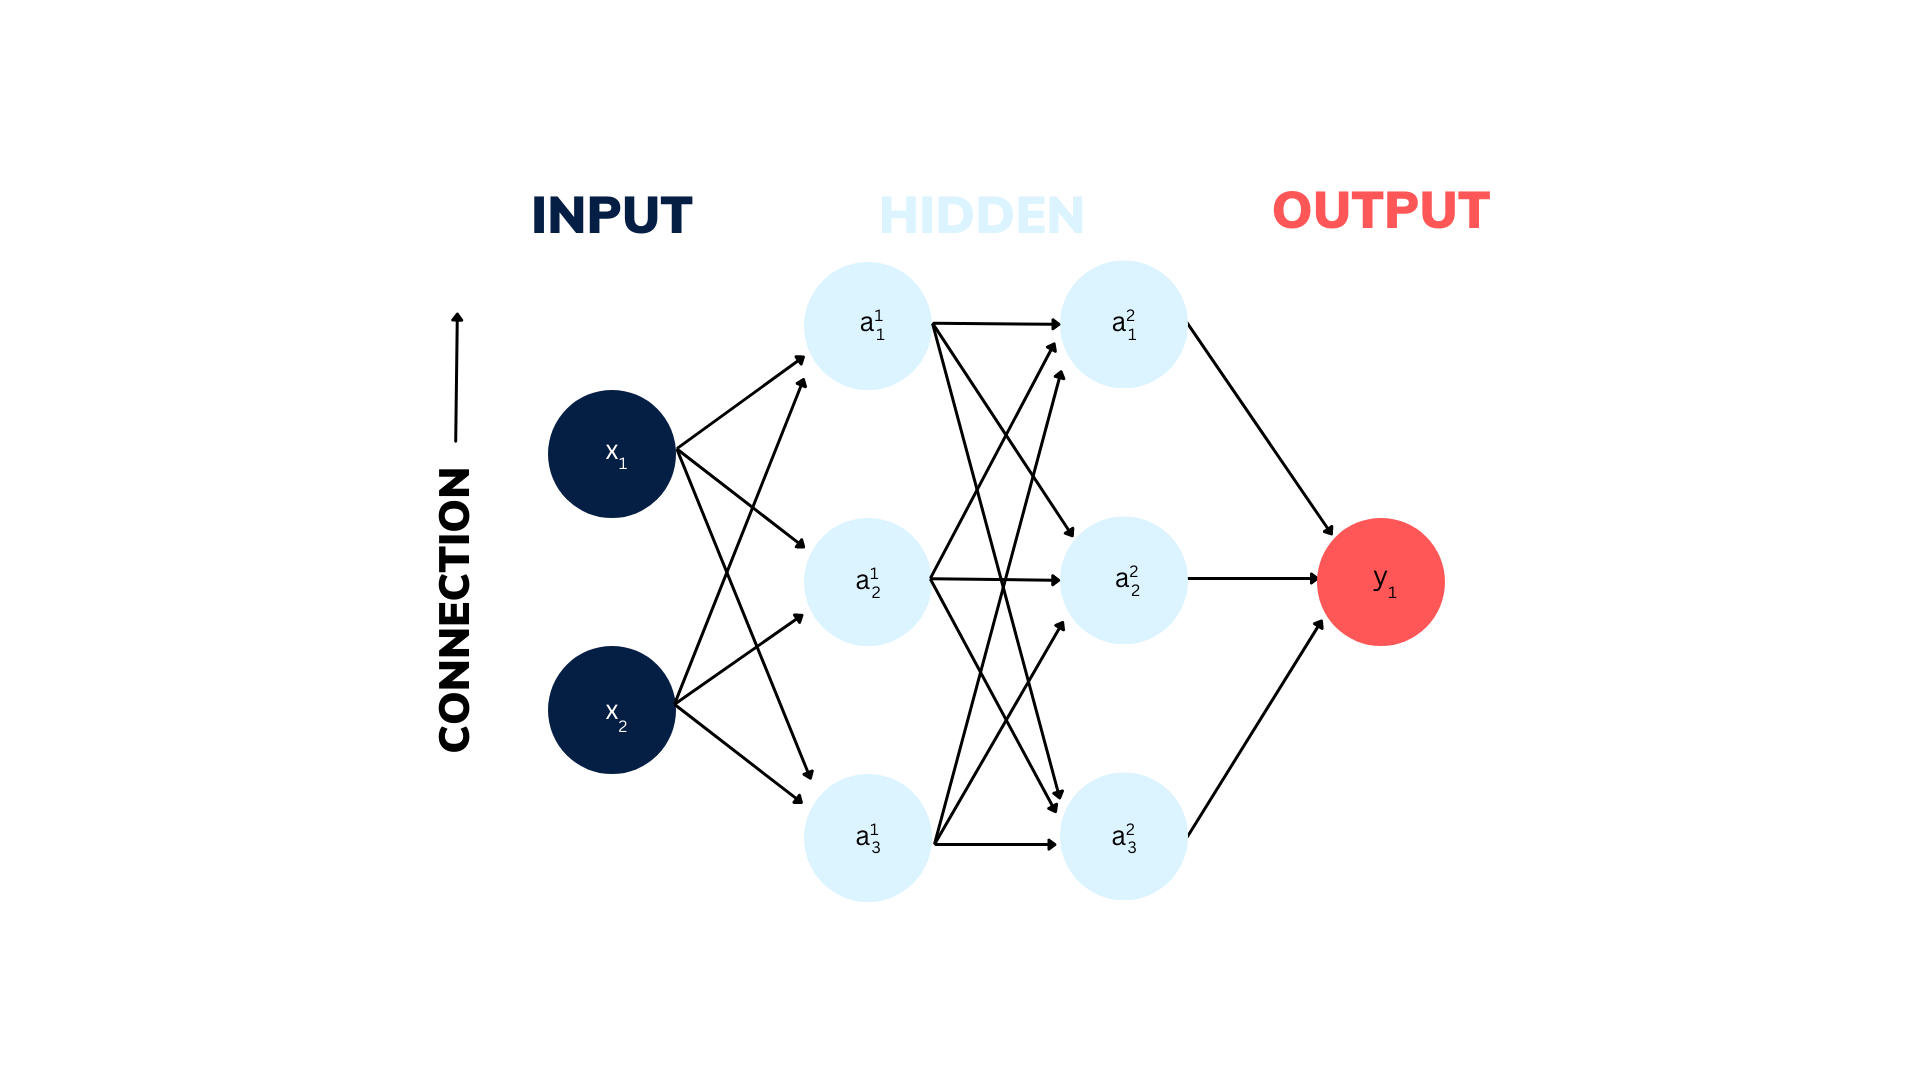
\includegraphics[width=0.9\textwidth]{Figures/Illustrations/Input_labels.png}
    \vspace*{-12.5mm} 
    \caption{An illustration of a \ac{NN} with two hidden layers.}
    \label{fig:NN}
\end{figure}
In figure \ref{fig:NN} we can see how all the different nodes are connected, illustrated by 
the arrows. The passing of values between different nodes are controlled by a set of weights and
bias parameters. These parameters are defined for each connection and are what will be tuned 
during training. The weights and biases for a given connection of two nodes, defines the effect on node 
has on the other.
\\
In a traditional \ac{FFNN} the information is passed linearly (in figure \ref{fig:NN}, from left to right) 
in a process we call \emph{forward-propogation}. Other variants can include the information taking a more 
complex route. It is often the route from input- to output-layer that categorizes the type of \ac{NN}. In 
this report I used a simple \ac{FFNN}. 

\subsubsection{Feeding Forward}\label{subsubsec:FP}
With the structure described in the previous section, a trained model, $\mathcal{F}$ produces a prediction,
$\bf{y}$ for a data set, $\bf{x}$ by passing information from input-layer, through all hidden-layers then
to output-layer, which we call forward-propagation. In this section I aim to explain the underlying algorithm and math
used by the \ac{NN} to map input to output. 
\\
We imagine the passing from hidden-layer $l-1$ to $l$, where $l \in \{2,...,N_L \}$\footnote{There is a special
case for when $l=1$ which will be addressed in the next paragraphs.} and $N_L$ is equal to the
number of hidden layers. The value of a node in layer $l$, is defined as $a^l_j$ (as indicated by figure \ref{fig:NN}), 
where $j\in \{0,1,...,N^l\}$ and $N^l$ is equal to the number of nodes in $l$. The value of $a_j^l$ is defined as 
the \emph{activated} sum of all nodes in the previous layer, $a_j^{l-1}$ where the sum is weighted by a parameter $\bf{w} \sf _j^l$ 
and scaled by the bias, $b^l_j$ for $j\in \{0,1,..., N_{l-1} \}$. The inactivated value of for a node j in layer l is defined as 
\begin{align}
    z_j^l = \sum_{k=1} ^ {N_{l-1}} w_{kj}^la_k^{l-1} + b^l_k,
\end{align}
where $w_{kj}^l$ corresponds to the weight in $\bf{w} \sf _k^l$ specific for the connection between node k and j.
\\
To attain the full activated value, $a_j^l$ we pass $z_j^l$ through the activation function. The activation function, $\sigma^l$ 
is a generally non-linear function used to control the limit or expand the value range for the node values. The activation 
function is general for all nodes in a given layer, but can vary in between layers. Therefore,
we find $a_j^l$ by the equation
\begin{align}\label{eq:ajl}
    a_j^l = \sigma \left (\sum_{k=1} ^ {N_{l}} w_{kj}^la_k^{l-1} + b^l_k\right ) = \sigma^l(z_j^l).
\end{align}
A more detailed illustration of the information pass from one layer to a node in the next is displayed 
in figure \ref{fig:WB}. In figure \ref{fig:WB}, we see all steps described in the process; \emph{(1)} all nodes in 
l-1 are summed with a corresponding weight, \emph{(2)} the sum is scaled by a constant term (bias), \emph{(3)} the 
scaled and weighted sum defines the inactivated value $z_j^l$, \emph{(4)} we define $a^l_j$ by passing the 
sum through $\sigma^l$.  
\begin{figure}
    \centering
    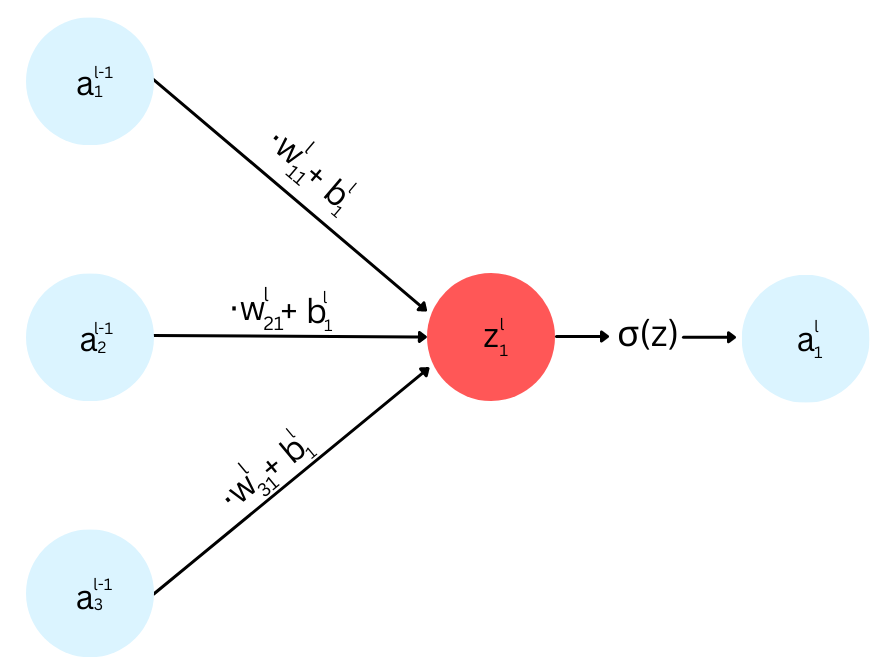
\includegraphics[width=0.5\textwidth]{Figures/Illustrations/WeightBias.png}
    \caption{An illustration information pass for one layer to another.}
    \label{fig:WB}
\end{figure}
This method is used for information pass between all layers, except the between the first and the second. 
In this case we simply replace the activated term, $a_k^{l-1}$ in equation \ref{eq:ajl}, by the input data,
$x_i$ for $i\in\{0,1,...,N\}$, where N is equal to the number features for the data. In the case $l=1$, \ref{eq:ajl} 
becomes
\begin{align}
    a_j^1 = \sigma \left (\sum_{k=1} ^ {N} w_{kj}^1x_k + b^1_k\right ) = \sigma(z_j^1).
\end{align}
In the case where $l=L$, $a_j^L$ is equal to the final output. 
\subsubsection{Back Propagation}\label{subsubsec:BP}
